\section{Experiments and Results}\label{sec:exp}
We conducted a set of experiments on real and synthetic data to evaluate our framework.
We designed our experiments to evaluate the following characteristics:
(1) Comparing \sampleclean with \biascorrected by varying the amount of each type of error (value, condition, duplication).
(2) Exploring the trade-off between result quality and cleaning cost provided by \sampleclean and \biascorrected.
(3) Measuring the required cleaning cost to achieve a certain accuracy by varying data size.
(4) Comparing with existing approaches that either clean all of data or none of data.
(5) Evaluating our framework on real datasets.


\subsection{Experimental Settings and Datasets}\label{subsec:dateset}
%We designed a simulation to represent the application of a data-cleaning technique and subsequent result estimation.
%As before, we support the following data-cleaning actions: repair the incorrect values in both aggregation and predicate attributes, and merging duplicate tuples.
We evaluate the efficacy of our approach with the following quantities: (1) \emph{Number of Cleaned Samples}. The number of tuples that are sampled and cleaned to produce an estimate; (2) \emph{Error \%}. An error \% of q\% signifies that with 95\% probability the estimate is within $\pm q\%$ of the true value. 

We refer to our framework \saqpplus as the one that can dynamically choose the better result between \biascorrected and \sampleclean. We compare \saqpplus with existing solutions that either clean none of the data (\alldirty) or clean all of data (\allclean). 
To compare different types of errors, we classify them by the error rate (the number of tuples affected by the error) ranging from 0\% (all of the tuples clean) to 100\% (all of the tuples dirty) for value, condition, and duplication errors.
%Accordingly, we use our datasets explore how different distributions of errors affect aggregate query results and our choice of estimation method.
%\item Cleaning Benefit: For $k$ cleaned samples, the benefit is the ratio of the error bound to data error percentage.
%For example, a cleaning benefit of $+30\%$ for 100 samples means that cleaning 100 samples means that the Error Bound is 30\% smaller than the original data error.
\begin{figure*}[t] \vspace{-2em}
\centering
\hspace*{-2em}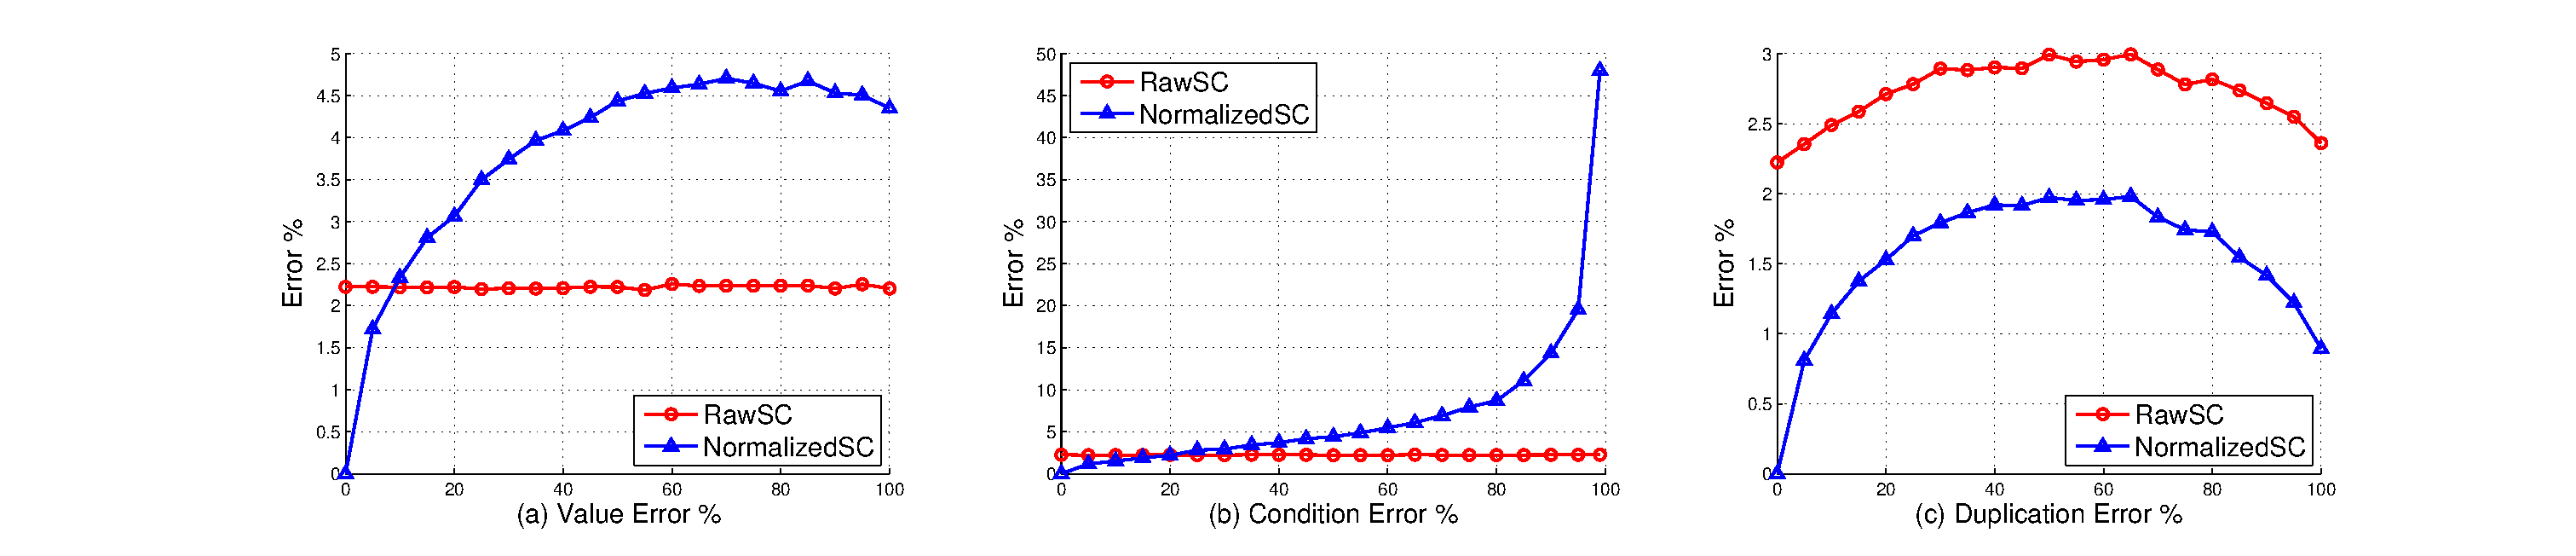
\includegraphics[scale=0.35]{exp/allerror-percent.eps}\\ \vspace{-1em}
%\small {(a)  \hspace{17em} (b)  \hspace{17em} (c)}
\caption{Varying the amount of each type of error on the TPC-H dataset and measured the performance of \bias vs. \sampleclean.}
\label{exp:all-errorpercent}
%\vspace*{-10pt}
\end{figure*}

\subsubsection{TPC-H Dataset} \label{exp:tpch}
We generated a 1GB TPC-H benchmark\footnote{\scriptsize http://www.tpc.org/tpch} dataset (6,001,199 Records in \texttt{lineitem} table).
The \texttt{lineitem} table schema simulates industrial purchase order records.
We used this dataset to model errors where the purchase orders were digitized using optical character recognition (OCR).
We denote a value-error percentage a\% as a\% of digits in the database were recognized as their most likely OCR false positive digit.
For condition errors, we simulated missing values by randomly selecting p\% of tuples and removing their predicate attribute.
We also randomly duplicated d\% of tuples with the following distribution: 80\% one duplicate, 15\% two duplicates, 5\% three duplicates.
%Accordingly, we use the following notation for TPC-H simulations (a\% value errors, p\% condition errors, d\% duplication errors).

For this dataset, we experiment with \avgfunc, \countfunc, and \sumfunc aggregations applied to this query:
\begin{alltt}
SELECT f(quantity) FROM lineitem
WHERE returnflag = `A' AND linestatus = `F';
\end{alltt}
which finds aggregate quantities of purchases that satisfy simulated conditions (returnflag = `A' and linestatus = `F').
In the clean data, there are 1,478,493 tuples satisfying the conditions that corresponds to a $24.6\%$ selectivity of this query.

\subsubsection{Microsoft Academic Search Dataset}
Microsoft maintains a public database of academic publications\footnote{\scriptsize http://academic.research.microsoft.com (Accessed Nov. 3, 2013)}.
The errors in this dataset are primarily duplicated publications and mis-attributed publications.
We selected publications from three database researchers: Jeffrey Ullman, Michael Franklin, and Rakesh Agarwal.
To clean a sample of publications, we first manually removed the mis-attributions in the sample. Then, we applied the technique used in~\cite{DBLP:journals/pvldb/WangKFF12} to identify potential duplicates for all of publications in our sample, and manually examined the potential matches.  
For illustration purpose, we cleaned the entire dataset, and showed the cleaning results in Table~\ref{tbl:dataset:ms-academic}. 
\begin{table}[!ht]\vspace{-1em}
\centering\caption{Microsoft Academic Search Dataset.}\vspace{.5em} \label{tbl:dataset:ms-academic}
\begin{tabular}{r r r r r}
\hline\hline
Name & Dirty & Clean & Pred \% & Dup \\ 
\hline  % inserts single horizontal line
Rakesh Agarwal & 353 & 211 & 18.13\% & 1.28\\
\hline
Jeffery Ullman & 460 & 255 & 05.00\% & 1.65\\
\hline
Michael Franklin & 560 & 173 & 65.09\% & 1.13\\
\hline
%\hline %inserts single line
\end{tabular}\vspace{-.75em}
%\reminder{May be we need to save some space.}
%\caption{The Microsoft Academic Search Dataset. We manually cleaned the datasets for each of the authors.
%This table shows the difference between the reported number of publications (AllDirty) and the number of publications after our cleaning (AllClean).
%We also include the false positive percentage and the duplication ratio (Section \ref{sec:sampleclean}) to illustrate the type of errors.}\label{dataset:ms-academic}\vspace{-1em}
\end{table}

This table shows the difference between the reported number of publications (Dirty) and the number of publications after our cleaning (Clean).
We also diagnosed the errors and recorded the duplication ratio (Dup) and the percentage of mis-attributed papers (Pred).
Both Rakesh Agarwal and Michael Franklin had a large number of mis-attributed papers due to other authors with the same name (64 and 402 respectively).
Jeffery Ullman had a comparatively larger number of duplicated papers (182).
%We chose this dataset since the errors are of the same order of magnitude as the data.

\subsubsection{Sensor Dataset}\label{exp:sensor}
We also applied our approach to a dataset of indoor temperature, humidity, and light sensor readings in the Intel Berkeley Research Lab.
The dataset is publicly available for data cleaning and sensor network research from MIT CSAIL\footnote{\scriptsize http://db.csail.mit.edu/labdata/labdata.html}.
We selected one month of readings and aggregated the values of all the sensors into a single aggregate reading for each minute in the month.
The resulting dataset had 44,460 sensor readings spaced one minute apart.
We applied algorithmic cleaning techniques (as opposed to manual cleaning) as described in~\cite{DBLP:conf/pervasive/JefferyAFHW06} to a sample of data.
%While many other cleaning techniques available for sensor data, the goal of this experiment is not to evaluate which cleaning technique performs better, but is to show that estimating results by cleaning a small number of samples could achieve much better results than those obtained from the entire dirty data. 

%\subsubsection{Entity Resolution Datasets}
%We applied our technique on datasets used to evaluate entity resolution systems~\cite{DBLP:journals/pvldb/KopckeTR10,DBLP:conf/kdd/BilenkoM03}.
%These datasets had only duplication errors and thus we used them to evaluate distinct count queries.
%Each of these datasets are illustrative examples of reasons why duplicate tuples occur in real data, and how these reasons affect the distribution of duplicates.
%We experimented with a dataset of 2173 products that was integrated from two different sources of information.
%As a result, there was 50.4\% duplication error with 1097 duplicates.
%We also evaluated dataset of restaurants which consisted of 858 tuples, 106 of which were duplicates (12.3\% duplication error); demonstrating datasets with a small amount of duplication error due to naming uncertainty.
%Finally, we applied our techniques to a dataset of 997 scholarly papers with a very large number of duplicates (806 duplicates, 80.8\% duplication error).
%Some of the papers in this dataset were duplicated over 50 times.

%\subsubsection{GoogleScholar Author Profile}
%We found that for some authors with common names or initials their GoogleScholar Author Profile lists publications which they did not write.
%This is a perfect dataset to demonstrate an estimation setting where there are many false positive errors.
%We highlighted one specific author, Wei Wang, whose profile lists 3000 publications.
%We then confirmed these publications with the publications on her home page \footnote{http://www.cs.ucla.edu/~weiwang/chrolist.html. Accessed October 12, 2013.}.
%We treat the confirmed papers as the ground truth dataset, and the rest as false postives errors (eg. papers that she did not write).
%Since, we were able to confirm a set of 125 papers on her homepage, the dataset has a very high false positive rate around 95\%.



\subsection{\sampleclean vs. \bias}
We evaluated \sampleclean and \bias for a fixed cleaned sample size, and for each type of error, we varied the error percentage.
This illustrates the regimes in which our framework will have good performance since we can apply the more accurate of the two approaches.
For all of our TPC-H experiments, we cleaned a fixed set of 10,000 samples (0.17\% of all tuples), and evaluated the performance on the \avgfunc query. 




%\begin{figure}[h]
%\centering
%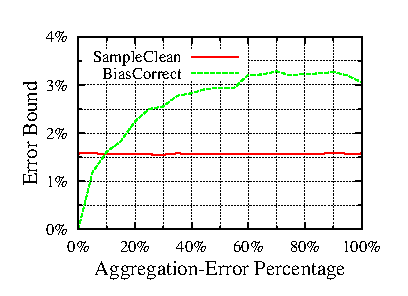
\includegraphics[scale=1]{exp/aggregation-errorpercent.eps}\\
%\caption{\sampleclean v.s. BiasCorrect by varying aggregation errors (Cleaned sample size = 5000)}
%\label{exp:aggregation-errorpercent}
%\vspace*{-10pt}
%\end{figure}

In Figure~\ref{exp:all-errorpercent}(a), we explored \avgfunc queries on tuples with only value errors.
We find that \bias gives results with narrower confidence intervals when the value errors are small.
\sampleclean, on the other hand, is actually independent of the value error rate as it only reports the aggregation of clean data.
Accordingly, since our framework dynamically chooses the more accurate approach, we can give tight bounds for datasets with higher and lower error rates.

%\begin{figure}[h]
%\centering
%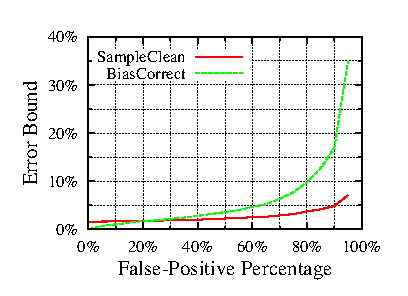
\includegraphics[scale=1]{exp/predicate-errorpercent.eps}\\
%\caption{\sampleclean v.s. BiasCorrect by varying false positive error rate (Cleaned sample size = 5000)}
%\label{exp:predicate-errorpercent}
%\vspace*{-10pt}
%\end{figure}



We repeat the same experiment with condition errors in Figure \ref{exp:all-errorpercent}(b) and observed similar behavior.
For small error rates, \bias gives a narrower confidence interval than \sampleclean, but \sampleclean returns a result that is not dependent on the rate of errors.
%If we clean a fixed set of tuples, the performance of \sampleclean is dependent on the selectivity of the query; since if the query is highly selective we need to take a larger random sample.
%However, if we have random condition errors that do not change the selectivity of the query, then \sampleclean is not affected.

%\begin{figure}[h]
%\centering
%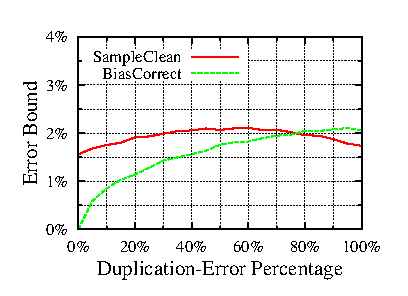
\includegraphics[scale=1]{exp/duplication-errorpercent.eps}\\
%\caption{\sampleclean v.s. BiasCorrect by varying duplication errors (Cleaned sample size = 5000)}
%\label{exp:duplicate-errorpercent}
%\vspace*{-10pt}
%\end{figure}

Figure~\ref{exp:all-errorpercent}(c) compares the \avgfunc query results of \sampleclean and \biascorrected on the data with duplication errors.
Consistent with all of our other experiments, \bias was more accurate when there were a small number of duplicates.
A counter-intuitive result is that the estimation error actually decreases after a point for both \sampleclean and \bias.
To better understand this phenomenon, suppose every tuple had exactly one duplicate, then \avgfunc query would be correct even on the dirty data.








\begin{figure}[t]
\hspace*{-2em}
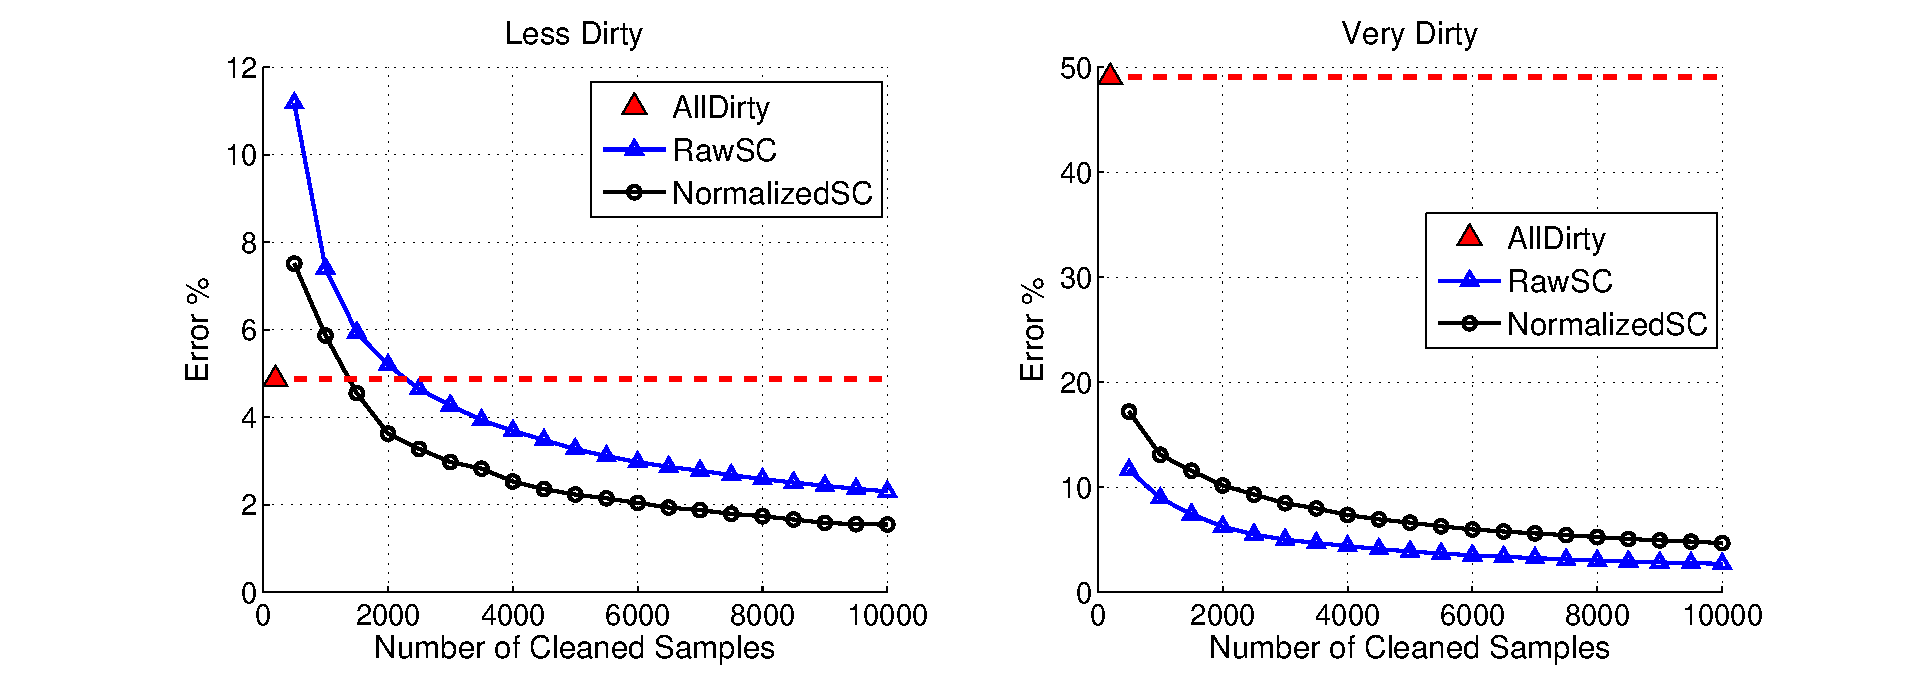
\includegraphics[scale=0.28]{exp/allerror-samplesize.eps}\vspace{-1em}
%\small {\hspace*{2em}(a) High Error Percentage  \hspace{3em} (b) Small Error Percentage}
\caption{Comparison of the convergence of the methods on two TPC-H datasets of 6M tuples with simulated errors (30\% value, 10\% condition, 20 \% duplication) and (3\% value, 1\% condition, 2\% duplication). On the dataset with larger errors, we find that \sampleclean gives a narrower confidence interval, and on the other \biascorrected is more accurate. }\vspace{-1em}
\label{exp:error-samplesize}
%\vspace*{-10pt}
\end{figure}

\subsection{Cleaning Cost v.s. Result Quality}
%One of our key motivations is to find the minimum number of samples to achieve a certain percentage of confidence. 


%\begin{figure}[t]
%\vspace{10pt}
%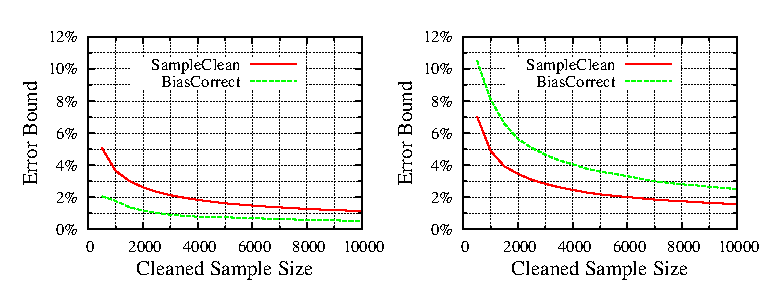
\includegraphics[scale=0.7]{exp/predicate-samplesize.eps}\\
%\small {\hspace*{2em}(a) 5\% False Positive Errors   \hspace{2em} (b) 50\% False Positive Errors}
%\caption{\sampleclean v.s. BiasCorrect by varying cleaned sample size (False Positive errors = 5\%, 50\%)}
%\label{exp:predicate-samplesize}
%\vspace*{-10pt}
%\end{figure}
%\begin{figure}[t]
%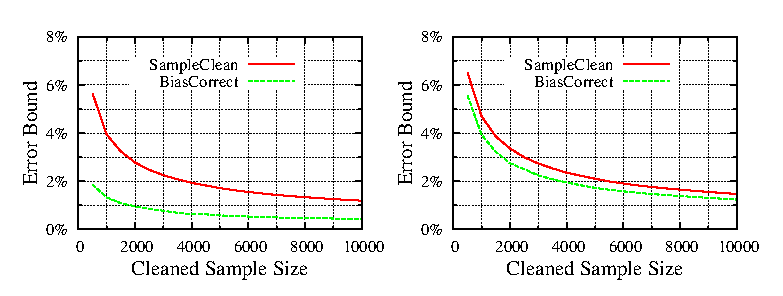
\includegraphics[scale=0.7]{exp/duplication-samplesize.eps}\\
%\small {\hspace*{2em}(a) 5\% Duplication Errors   \hspace{2em} (b) 50\% Duplication Errors}
%\caption{\sampleclean v.s. BiasCorrect by varying cleaned sample size (Duplication errors = 5\%, 50\%)}
%\label{exp:duplication-samplesize}
%\vspace*{-10pt}
%\end{figure}

We evaluated how the number of cleaned samples affects the result error for \sampleclean and \bias.
We ran the \avgfunc query on the two TPC-H datasets that we considered before: one where the percentages for each error type were (30\%,10\%,20\%), and one where each was (3\%,1\%,2\%).
Our results are shown in Figure \ref{exp:error-samplesize}.

Both of the methods converge at a rate $\frac{1}{\sqrt{K}}$ with respect to the sample size.
We can easily estimate how many samples we need to clean to achieve a specified error. %. %\sampleclean performs better on the data with less error while For the data set with more errors,
Another key insight is that since both converge at the same rate with respect to the sample size, the lines will never cross.
Consequently, there will always be a single \emph{better} choice between \sampleclean and \bias, and we do not have to worry about our choice being suboptimal for more cleaned samples.

We also compare our approaches with \alldirty. We can see both \sampleclean and \biascorrected can achieve a better result by cleaning only a small number of samples. Section~\ref{subsec:end-to-end} contains a more detailed comparison with \alldirty and \allclean.
%However, it is important to not the value to which each of these methods converge.
%We can see that \sampleclean and \bias converge to the AllClean value, while SampleDirty converges to the AllDirty value.




\begin{figure*}[t]\vspace{-2em}
\centering
\hspace*{-2em}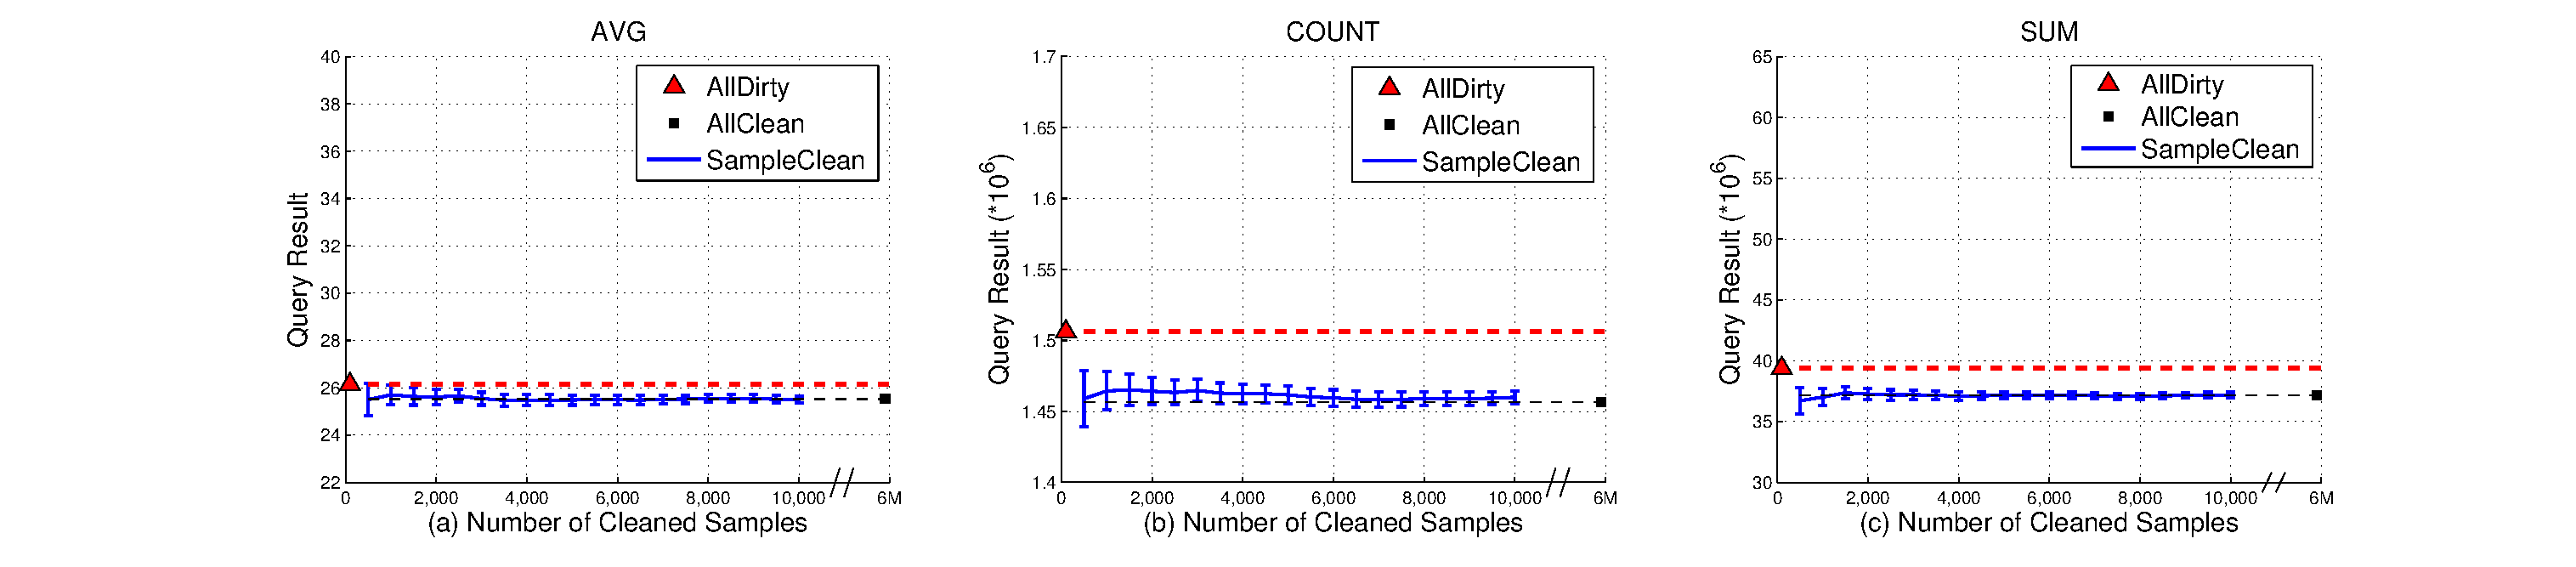
\includegraphics[scale=0.35]{exp/pk-alldirty-small-errors.eps}\vspace{-1em}
%\small {\hspace*{0em}(a) AVG Query   \hspace{10em} (b) COUNT Query  \hspace{7em} (c) SUM Query}
\caption{TPC-H evaluation with 3\% Value Error, 1\% Condition Error, 2\% Duplication Error on 6M tuples.
Our technique can efficiently estimate on datasets with a small number of errors due to the trade-off between \sampleclean and \bias.}
\label{exp:end-to-end-small}
%\vspace*{-10pt}
\centering\vspace{.5em}
\hspace*{-2em}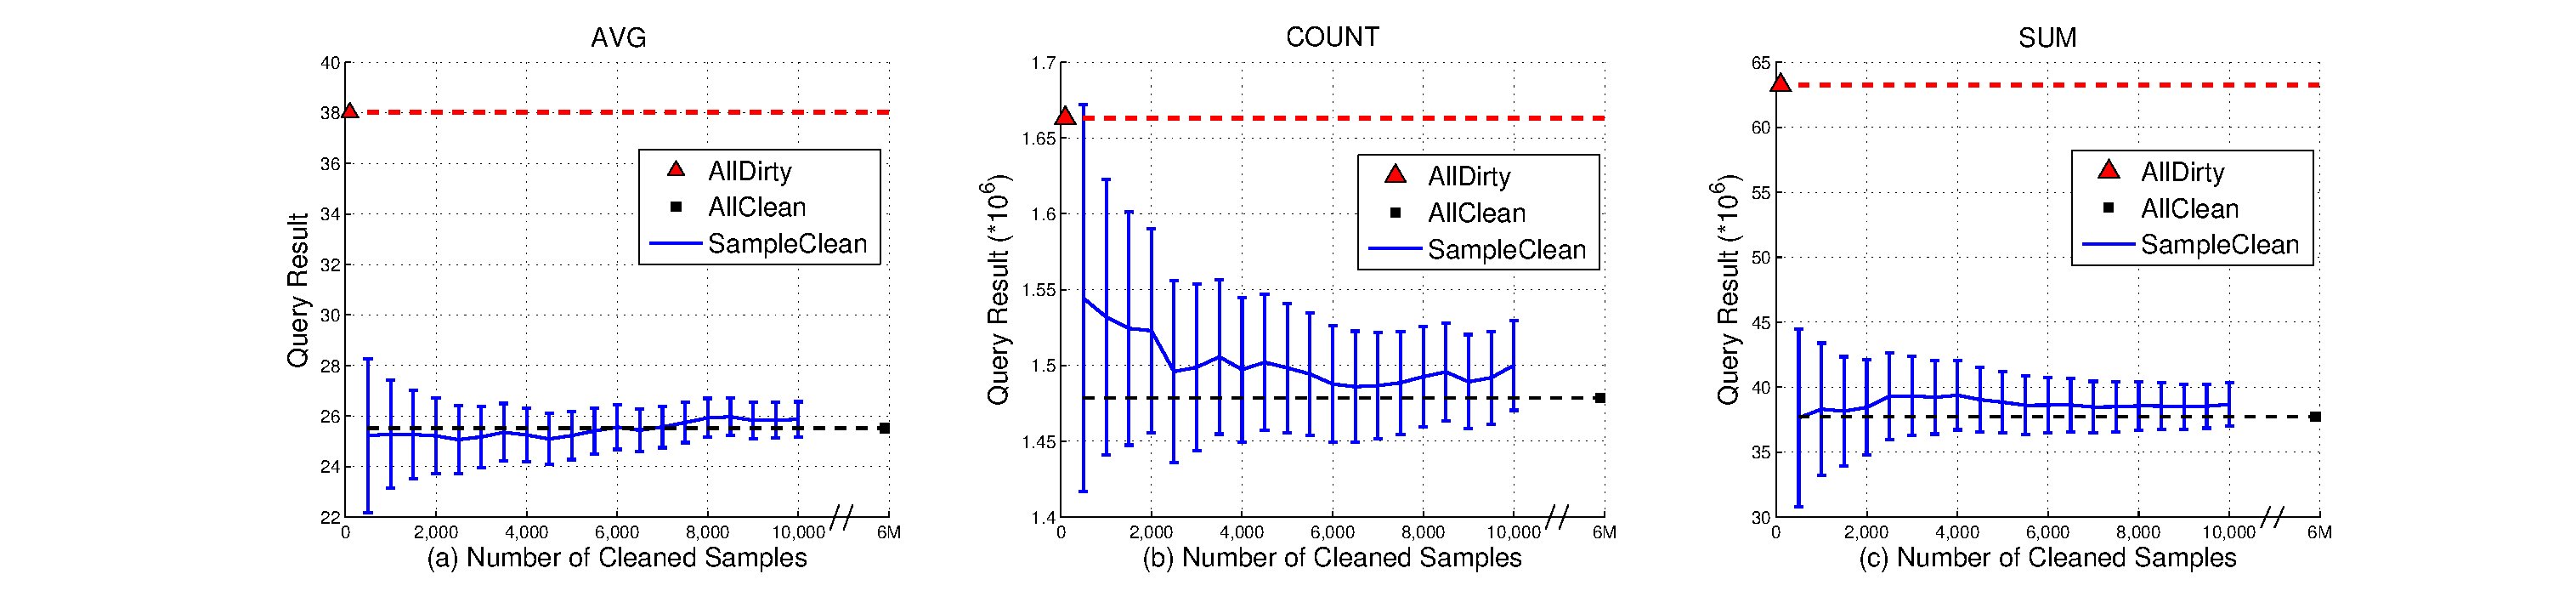
\includegraphics[scale=0.35]{exp/pk-alldirty.eps}\vspace{-1em}
%\small {\hspace*{0em}(a) AVG Query   \hspace{10em} (b) COUNT Query  \hspace{7em} (c) SUM Query}
\caption{TPC-H evaluation with 30\% Value Error, 10\% Condition Errors, 20\% Duplication Error on 6M tuples.
We find that even for a small number of cleaned samples, we can return results with high confidence.
We are able to achieve 95\% accuracy after cleaning only 0.08\% of the total samples.
%High rates of certain types of random errors, such a duplication, may start to cancel out bias.
%For example, if all of the tuples are duplicated exactly once then there is no need to clean duplicates. 
}
\label{exp:end-to-end}
%\vspace*{-10pt}
\end{figure*}



\subsection{Scalability of Cleaning Cost}

In our \sampleclean and \bias approaches, we return confidence intervals that are independent of the size of the dataset.
In terms of tuples cleaned, there is no difference between evaluating our approach on a 1GB dataset or on a 1TB dataset.
In Figure \ref{exp:scalability-size}, we show that if we simulate the 30\%, 10\%, 20\% errors in different sized TPC-H datasets (1GB, 10GB, 100GB, 1TB) as before, the number of cleaned tuples needed for a certain accuracy remains roughly constant.
Each dataset was generated in the same way; the errors were simulated from the same distribution.
It underscores that the number of samples needed to get a good estimate is a property of the variance of the data and its errors.

\begin{figure}[h]\vspace{-.5em}
\centering
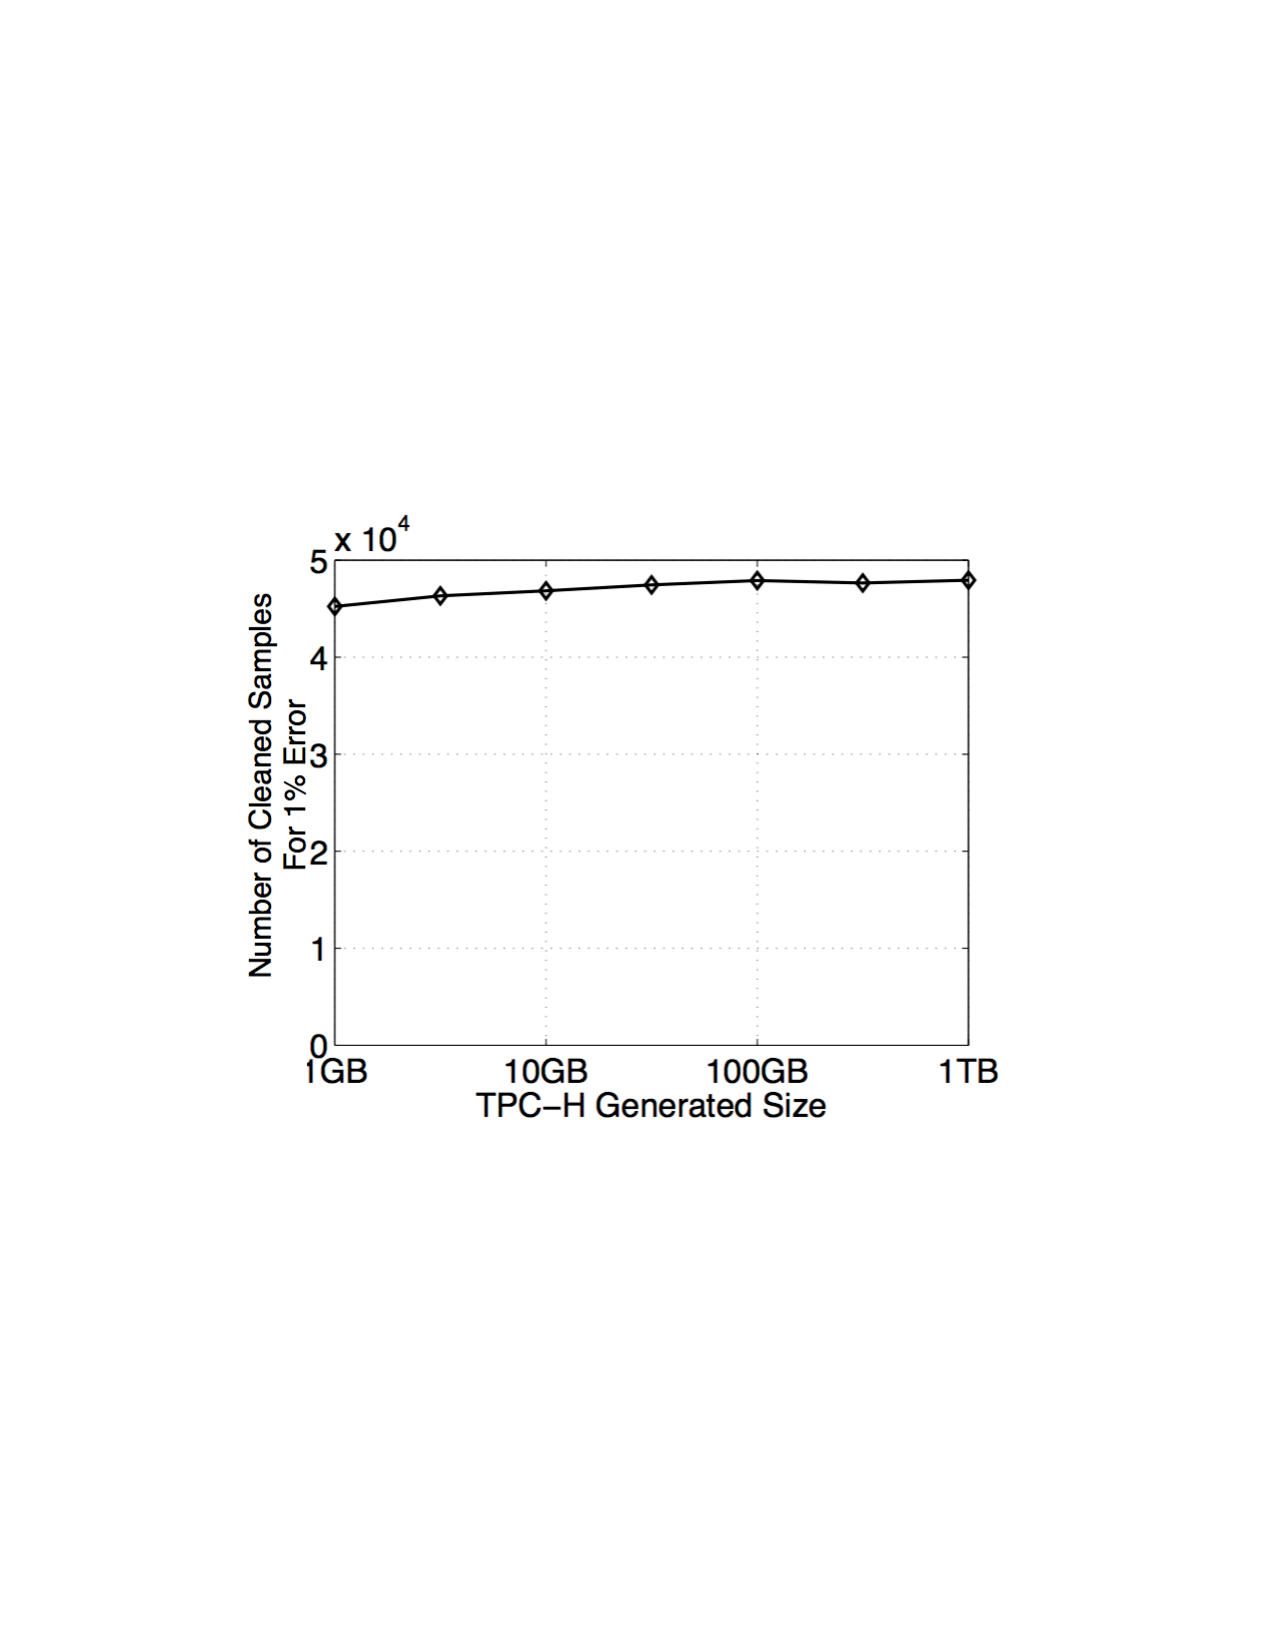
\includegraphics[scale=.4]{exp/scalability-size-cleaning.pdf}\vspace{-1em}
\caption{Scalability of \saqpplus on TPC-H (30\%,10\%,20\%) of different sizes. The number of cleaned tuples needed to achieve a certain accuracy does not increase with the size of the dataset.}\vspace{-.5em}
\label{exp:scalability-size}
%\vspace*{-10pt}
\end{figure}

\begin{figure*}[t]\vspace{-1em}
\centering
\hspace*{-2.5em}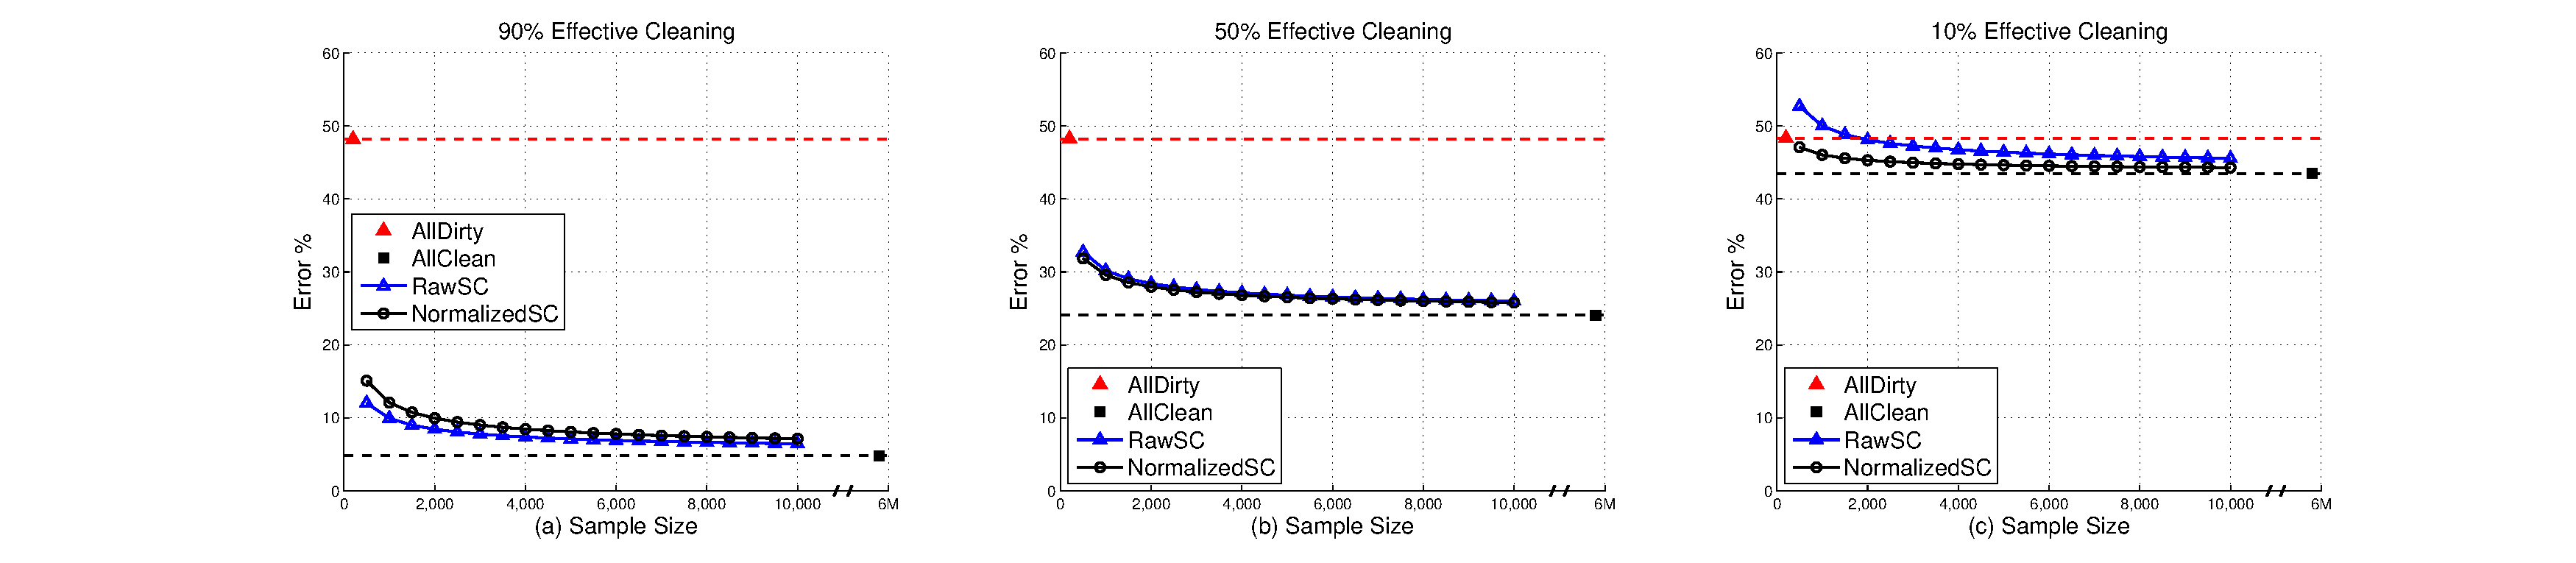
\includegraphics[scale=0.31]{exp/imperfect-cleaning-samplesize.eps}\vspace{-1em}
\caption{Imperfect Data Cleaning on TPC-H (30\%, 10\%, 20\%) of 6M tuples. 
Even with a data cleaning technique that is not always correct, we find that our results rapidly converge to the \allclean values.
We found that a 10\% effective cleaning module can give more accurate results than \alldirty with a sample size of 0.03\% of the dataset.}
\label{exp:imperfect}\vspace{-1em}
\end{figure*}



\subsection{End-to-End Experiment}\label{subsec:end-to-end}
We tested the end-to-end performance of the \saqpplus framework on a TPC-H dataset with small errors: 3\% value, 2\% duplication, and 1\% condition errors.
Under these errors, we evaluated the \avgfunc, \sumfunc, and \countfunc aggregations and compared the performance of our framework with \allclean and \alldirty in terms of result quality and cleaning cost.
To process the queries (refer to Section \ref{exp:tpch}), we uniformly sampled from the dataset.
Our results in Figure \ref{exp:end-to-end-small} suggest that \saqpplus quickly converges to the right answer, giving a flexible trade-off between tuples cleaned and the size of the confidence interval in the estimate.
We found that after cleaning only 1000 tuples (0.016\%), we were to estimate more accurately than \alldirty.



This was a dataset with small errors (mostly clean), and we wanted to understand how \saqpplus performs on a much dirtier dataset.
We repeated experiment under 30\% value, 20\% duplication, and 10\% condition errors (Figure~\ref{exp:end-to-end}).
On this dataset \alldirty differs from \allclean by 52\% in the \avgfunc function.
The results in Figure \ref{exp:end-to-end} show that \sampleclean still rapidly converges to the true values and outperforms \alldirty.
In addition, for all queries, our estimate is within 5\% of \allclean after cleaning only 5000 tuples (0.08\% of the total data).

Due to the trade-off between \bias and \sampleclean, we can estimate accurately for datasets that are both mostly clean or very dirty.
On the dataset with small errors, \bias was the more accurate estimation method and \sampleclean was more accurate on one in the presence of larger errors.
%Our technique is scalable since for both \sampleclean and \bias,
%we return confidence intervals that are independent of the size of the dataset.
%These confidence intervals are only dependent on the size of the sample, and the variance of the data.
%The number of samples needed to get a good estimate is really a property of the data and its errors, and not the size of the dataset.


\begin{figure*}[t]\vspace{-2.5em}
\hspace*{-2em}
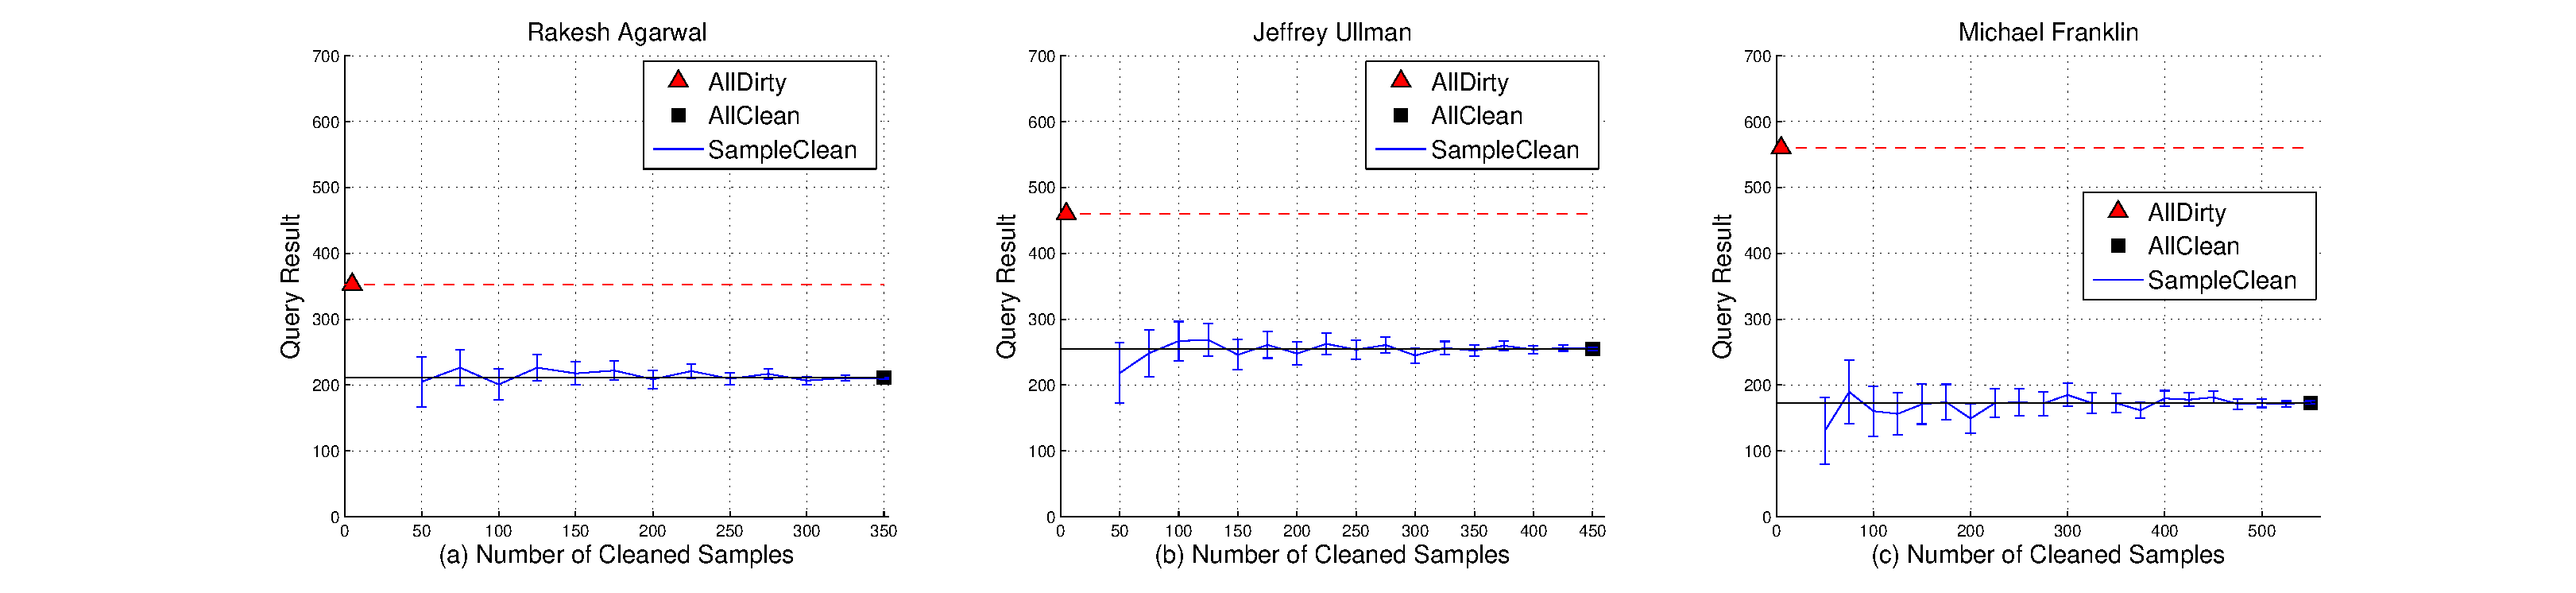
\includegraphics[scale=0.35]{exp/msacademic-paper-count.eps}\vspace{-1em}
\caption{The output of our result estimation framework for each author. The dataset was particularly dirty and cleaning only 50 tuples per author was sufficient to outperform an aggregation of the entire dataset.}
\label{exp:ms-academic-paper-count}
\end{figure*}

\subsection{Imperfect Data Cleaning}
\label{exp:sensitivity}

%Our approach is general enough to incorporate data cleaning that is imperfect (an \allclean result does not correspond to a true value).
%The confidence intervals we provide are with respect to \allclean and not dependent on knowing the true values.
In Figure \ref{exp:imperfect}, we experimentally show that \saqpplus is valuable even when the cleaning is incomplete.
We ran our experiments on a dataset with 30\% Value Errors, 10\% Condition Errors, and 20\% Duplication Errors, and simulated
a data cleaning technique that can only identify and clean a fixed percentage of errors.
We compared the Error \% of the query and the total sample size including tuples where the data cleaning failed.

Even though our estimates are now biased with respect to the true values, they are still unbiased with respect to \allclean.
Consequently, we found that even if our cleaning technique can clean only 10\% of the errors, we still only have to sample 2,000 tuples to achieve a more accurate result than \alldirty.
Furthermore, we can take advantage of both \sampleclean and \biascorrected.
If a technique changes a lot of the tuple values, then \sampleclean gives us a more precise estimate.
However, if a technique keeps most of the values the same \biascorrected is more precise.




\begin{figure}[t]\vspace{-1.8em}
\centering
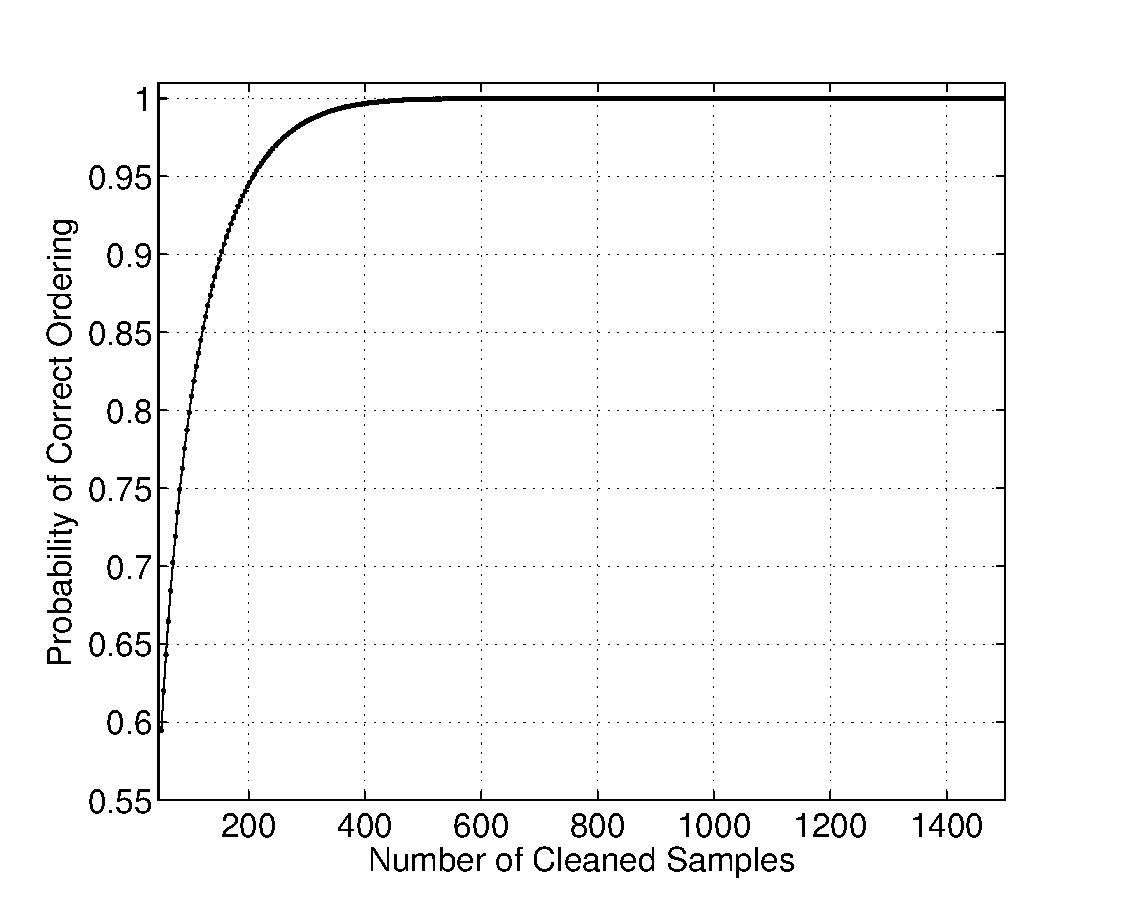
\includegraphics[scale=0.3]{exp/msacademic-paper-ranking.eps}
\caption{Even though \alldirty always returns an incorrect ranking, we can return the correct ranking with 95\% probability after cleaning only 210 total samples. To achieve a correct ranking with 99\% probability, we require 326 samples to be cleaned.}\vspace{-1em}
\label{exp:ms-academic-ranking}
\end{figure}

\subsection{Evaluation on Real Data}
The following sections contain experiments on two real datasets: Microsoft Academic Search and the Intel Lab Sensors.
As described in Section~\ref{subsec:dateset}, they contain different types of errors: the sensor dataset consists of predominantly value and condition errors, and the publication dataset consists of condition and duplication errors.

\subsubsection{Microsoft Academic Search}\label{exp:mas}
We designed this experiment to be illustrative of assessing the confidence of decisions based on dirty data, by trying to get an accurate publication count for the 
three authors.
We can see that in Table~\ref{tbl:dataset:ms-academic} AllDirty not only returns incorrect values but also returns an incorrect ranking of the three authors.
This is an example of a dataset where the data cleaning is quite well defined, we can apply our domain expertise in database publications to reason about each tuple in the dataset, but cleaning is very time consuming. 
In Figure \ref{exp:ms-academic-paper-count}, we show how our approach can budget data cleaning for each author up-to a desired query quality.
We clearly see that our estimates are centered around the AllClean value and even with the confidence intervals outperform aggregations of the full dirty data.

However, we do notice that the confidence intervals for the estimated paper counts overlap for a small number of cleaned samples.
We evaluated how many tuples would need to be cleaned to get an accurate ranking using a simulation; that is if we re-ran the same experiment with the same sample size what is the probability our ordering of the authors is accurate.
For each author, we treat the estimate of their paper count as a normally distributed random variable.
From these distributions, we sample 10000 paper counts and calculate the empirical probability of an incorrect ordering.
In Figure \ref{exp:ms-academic-ranking}, we show how we can return the correct ranking with 95\% probability after cleaning only 210 total samples.
To achieve a correct ranking with 99\% probability, we require 326 samples to be cleaned.
In comparison, AllDirty always returns an incorrect ranking.
\saqpplus provides a flexible way to achieve a desired confidence on decision based on dirty data queries.



\subsubsection{Sensor Dataset}
\begin{figure*}[t]\vspace{-2.5em}
\hspace{-60pt}
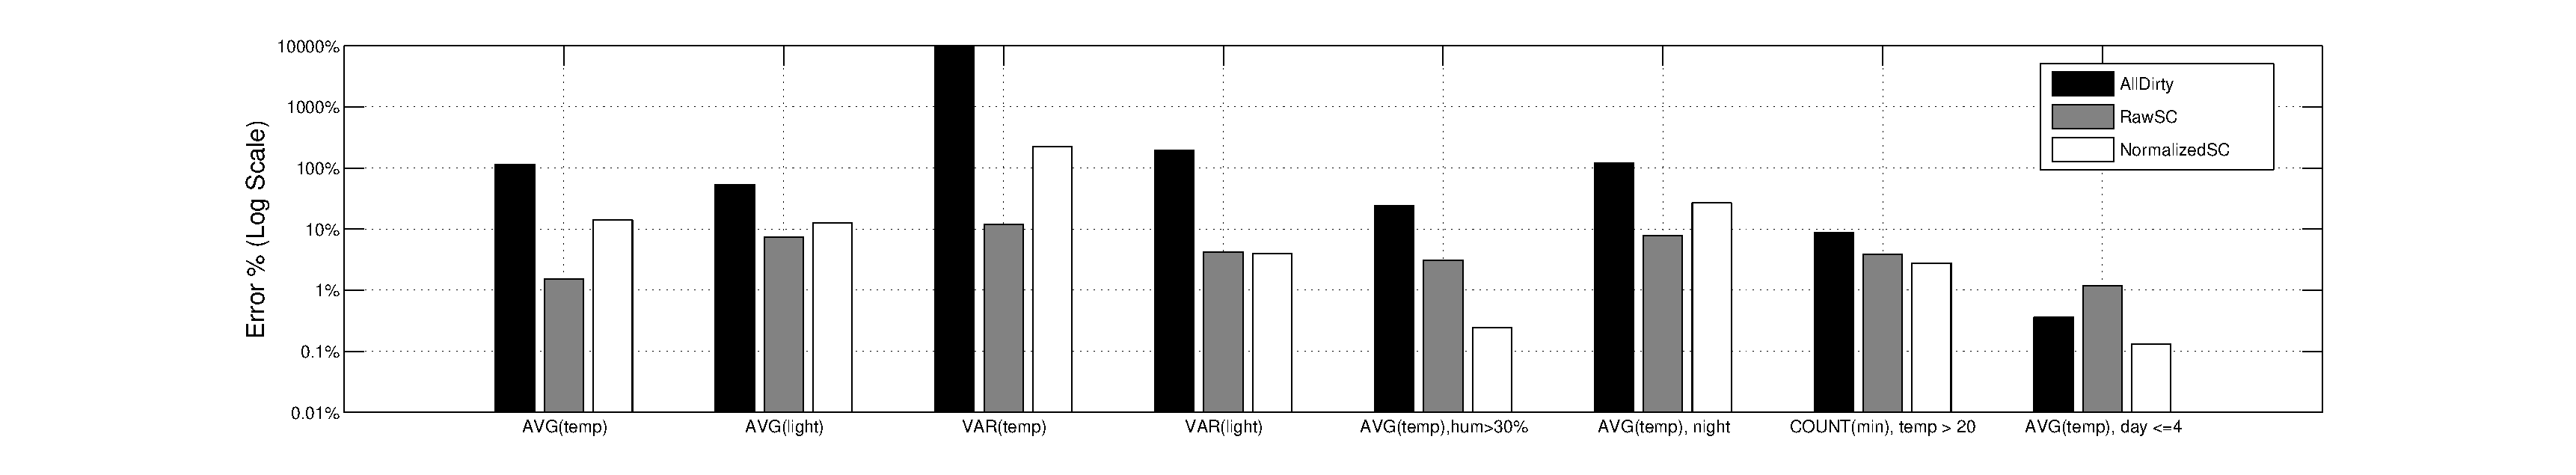
\includegraphics[scale=0.375]{exp/sensor-all-queries.eps}\vspace{-1em}
\caption{Queries applied to the sensor dataset. We applied a set of queries with a fixed sample (same for all queries) of 500 cleaned tuples. We compare the error percentage (log-scale) of AllDirty, \sampleclean, and \bias with respect to AllClean.
 For all of these example queries, we are able to achieve a relative error of less than $\pm 10\%$ even when the data error is orders of magnitude higher.}\vspace{-1em}
\label{exp:sensor-all-queries}
\end{figure*}
The sensor dataset consists of readings from inexpensive battery-operated sensors.
The failure mode of these sensors is returning incorrect readings, particularly when the available battery power is low.
We limited the dataset to a single month where the readings from the beginning of the month were largely accurate, while the readings from later in the month became increasingly inaccurate.
We cleaned 500 samples (1.12\%) of the dataset using the algorithm described in~\cite{DBLP:conf/pervasive/JefferyAFHW06} and applied a variety of queries to illustrate how different types of value and condition errors can affect results (Figure \ref{exp:sensor-all-queries}).

Like the TCP-H results, this experiment shows how having both \sampleclean and \bias helps us estimate accurately in different error distributions.
Surprisingly, we found that different queries on the same dataset may have very different error characteristics making the choice between \sampleclean and BiasCorrect very important.
From this experiment, we can also see the interactive latency capabilities of \saqpplus.
Since we cleaned the 500 sampled tuples, subsequent \sampleclean queries only need to operate on the cleaned sample.
This demonstrates how \sampleclean can give a very fast response time on large datasets as it only has to process the tuples in the cleaned sample.

The first two queries \texttt{avg}(temp) and \texttt{avg}(light) illustrate the severity of the sensor errors.
Simply taking an average over the dirty data results in an estimate that differs from AllClean by about 100\%.
However, for the cost of cleaning only 500 samples, we are able to achieve a confidence interval of $\pm 1.5\%$ and $\pm 15.2\%$ respectively.
Due to the nature of the sensor errors, a similar, but more dramatic, improvement is seen for \texttt{var}(temp) and \texttt{var}(light).
Random errors such as ones generated by electronic sensors tend to increase variance of the data, and we can see that our estimate for \texttt{var}(temp) is three orders of magnitude closer to AllClean.

We also evaluated the queries with predicates.
In the first query, we looked at the average temperature when the humidity was above 30\%.
For this query, there were both value and condition errors.
We also looked at the average temperature when the predicate attribute (time) was accurate even during sensor failures.
We found that our technique works well in both cases giving significant improvements over aggregations of the dirty data.

Finally, we demonstrate a query where the errors are relatively small.
We counted the number of readings where the temperature was above some threshold.
We found that the dirty aggregation was not very much worse than the confidence intervals returned by our method.
Furthermore, we also experimented with the average temperature over the first four days when most of the sensors were working.
In this query, AllDirty differed from AllClean by less than 1\%. 
In fact, AllDirty outperforms \sampleclean for 500 cleaned samples.
However, due to our tradeoff between \sampleclean and \bias, we are still able to improve on already good estimates.

%\subsubsection{MSAcademic/GoogleScholar Dataset}

%\begin{table*}[ht]
%\tiny
%\caption{For each example query we simulated the benefit of cleaning the MSAcademic/GoogleScholar Dataset. We report the Data Error, and the number of samples that need to be cleaned to achieve an 25\%, 50\%, and 75\% reduction in this error.}
%\label{exp:citations}
%\centering 
%\begin{tabular}{c c c c c c}
%\hline\hline
%No. & Query & Dirty Data Error & +25\% acc. &+50\% acc. & +75\%acc. \\ 
%\hline  % inserts single horizontal line
%1 & SELECT \textsf{AVG}(citation) FROM publication& 71.03\% & 28 & 105 & 577 \\
%2 & SELECT \textsf{SUM}(citation) FROM publication& 71.03\% & 28 & 105 & 577 \\ 
%3 & SELECT \textsf{COUNT}(citation) FROM publication& 3.96\% & 85 & 186 & 585 \\
%\hline  % inserts single horizontal line
%4 & SELECT \textsf{COUNT}(citation) FROM publication WHERE citation $\ge$ 50 & 56.35\% & 37 & 90 & 341 \\
%5 & SELECT \textsf{AVG}(citation) FROM publication WHERE citation $\ge$ 50 & 48.65\% & 370 & 723 & 1441 \\
%6 & SELECT \textsf{COUNT}(citation) FROM publication WHERE citation == 0 & 71.84\% & 132 & 283 & 811 \\
%\hline  % inserts single horizontal line
%7 & SELECT \textsf{COUNT}(citation) FROM publication WHERE year > 1980 & 3.55\% & 153 & 302 & 945\\
%8 & SELECT \textsf{COUNT}(citation) FROM publication WHERE year > 1980 *& 3.55\% & 1450 & 1725 & 2000\\
%9 & SELECT \textsf{AVG}(citation/(2013-year)) FROM publication & 69.31\% & 34 & 76 & 381\\
%\hline %inserts single line
%\end{tabular}
%\end{table*}

%We applied our framework on this dataset of paper citations.
%The experiment considers the data as a single table \textbf{publication} with the attributes \textbf{citation} (number of citations received by the paper) and \textbf{year} (the year of publication).
%We assume that there are only errors in the \textbf{citation} attribute.
%We present a set of 9 example queries and their results (Table \ref{exp:citations}).
%For each query, we evaluated what the uncleaned result would be, then calculated the number of clean samples needed to out perform a dirty aggregation by 25\%, 50\%, and 75\%.

%Our results illustrate that a naive aggregation of the dirty data (eg. Query 1) could result in an estimate is more than 70\% away from the true value.
%If we take the Query 1 as an example, even for a relatively small number of cleaned tuples (about 5\% of the data) we can reduce this error by 50\%.

%It is important to note the errors in this dataset are not independently random errors.
%We can see indications of strong systemic error in comparing the quality of Query 3 and Query 4.
%It is clear that papers with a larger number of citations were more likely to be duplicated.
%In addition, we see that there is a complex dependency of the quality of an estimate and the data and error variance.
%If we compare Query 4 and Query 5, we see that the simple change of aggregation function requires much more cleaning for similar accuracy.

%We can also experiment with more complex multi-attribute queries.
%In Query 7 and Query 8, we illustrate a point about dealing with combinations of errors and best practices when executing these queries.
%Query 7 counts the number of papers in the dataset published after 1980, and not surprisingly the results are similar to that of Query 1; where the only source of error is a small duplication error.
%However, Query 8 executes the same count in a different way.
%If we treat the entire set of papers as our population, and mark those that were published before 1980 as false positives we can still get an unbiased estimate.
%However, setting many elements to zero in $\phi_f(.)$ increases the variance of the estimate and we require many more cleaned tuples to answer the same query.
%This is related to the point made in Section \ref{sec:optimization}, where we skip false positives in the mean query to reduce estimate variance.

%Finally, we demonstrate the performance on a multi-dimensional query.
%Query 9 calculates the average number of citations per year received by the papers in the dataset.

%\subsubsection{GoogleScholar Author Profile}
%\begin{figure}[t]
%\centering
%\hspace*{-2em}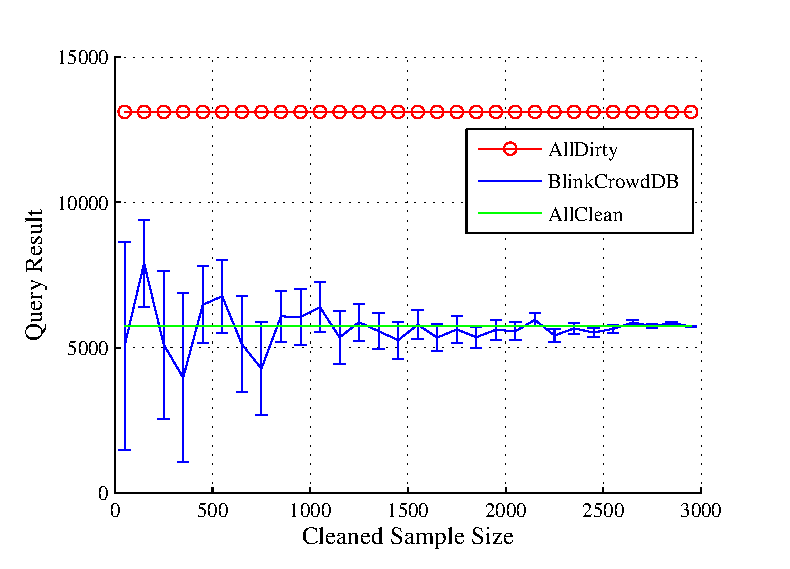
\includegraphics[scale=0.45]{exp/false-positive-error-weiwang.eps}\\
%\caption{We estimated the total number of citations for confirmed publications on the dirty dataset from the author's GoogleScholar Author Profile. We were unable to confirm over 95\% of the publications, and treated those as false positive errors.}
%\label{exp:wei-wang-fp}
%\vspace*{-10pt}
%\end{figure}
%Given this profile dataset with a very high false positive rate, we tried to estimate the total number of citations received by the author.
%The sum over all the confirmed publications is 5735 citations, while over the entire dataset it is 13108.
%Our results in Figure \ref{exp:wei-wang-fp}, show that we easily outperform an aggregation of the full dirty data.
%For even 50 cleaned samples our error bound is less than the data error.

%However, if we measure error with respect to the true value we do require a lot more cleaning.
%For example, if we want to get within 10\% of the true value, we require 1406 sample cleaned.
%With a 95\% false positive error, this is an inherently hard dataset to estimate, and as a result we have to clean a large number of samples to get accurate estimates.

%\subsubsection{Entity Resolution Datasets}
%\begin{figure*}[t]
%\centering
%\hspace*{-5em}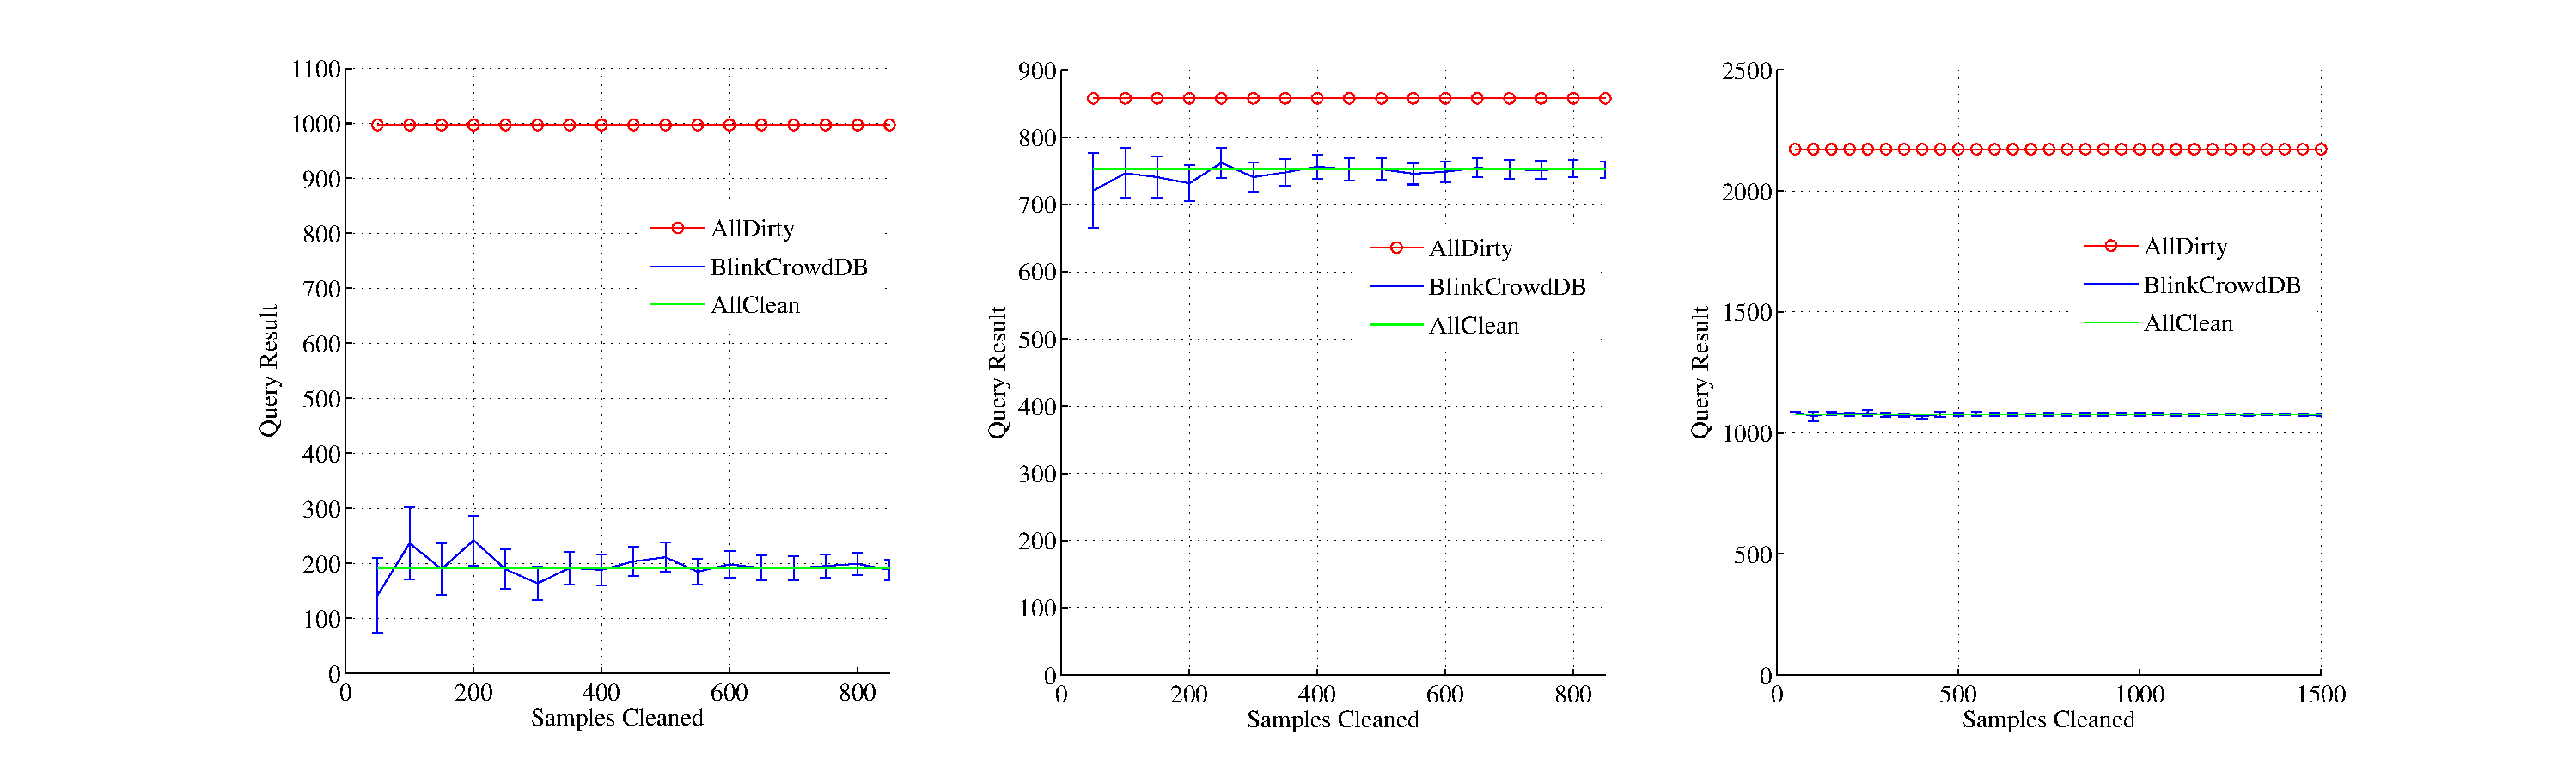
\includegraphics[scale=0.40]{exp/entity-resolution.eps}\\
%\small {\hspace*{1em}(a)Papers \hspace{11em} (b)Restaurants  \hspace{11em} (c)Products}
%\caption{We evaluate the \textbf{COUNT} query on three datasets with duplication errors. Our results show that even for a small sample of cleaned data tuples
%our estimates are relatively close to the true value.}
%\label{exp:entity-res}
%\vspace*{-10pt}
%\end{figure*}

%We applied our framework to the three entity resolution datasets to answer a count of the number of distinct elements (Figure \ref{exp:entity-res}).
%The results suggest good estimates on datasets with large number of duplicates as well as ones with a relatively small number of duplicates.
%It is interesting to note that we see that even sampling 100 or 200 clean tuples can result in a much better estimate than an exact aggregation of the dirty data.
%Another interesting point is in datasets such as the product dataset, where almost every tuple has 1 duplicate, the sample variance of our transformed data sequence
%is small resulting in very accurate estimates.
%This illustrates a key point that small duplication errors may be harder to handle than large number of duplicates.
%\reminder{Use my gnuplot template, and change the starting value of the y-axis to zero for each subfigure.}

%\subsection{Group By and Constrained Queries}
%\begin{figure}[t]
%\centering
%\hspace*{-2em}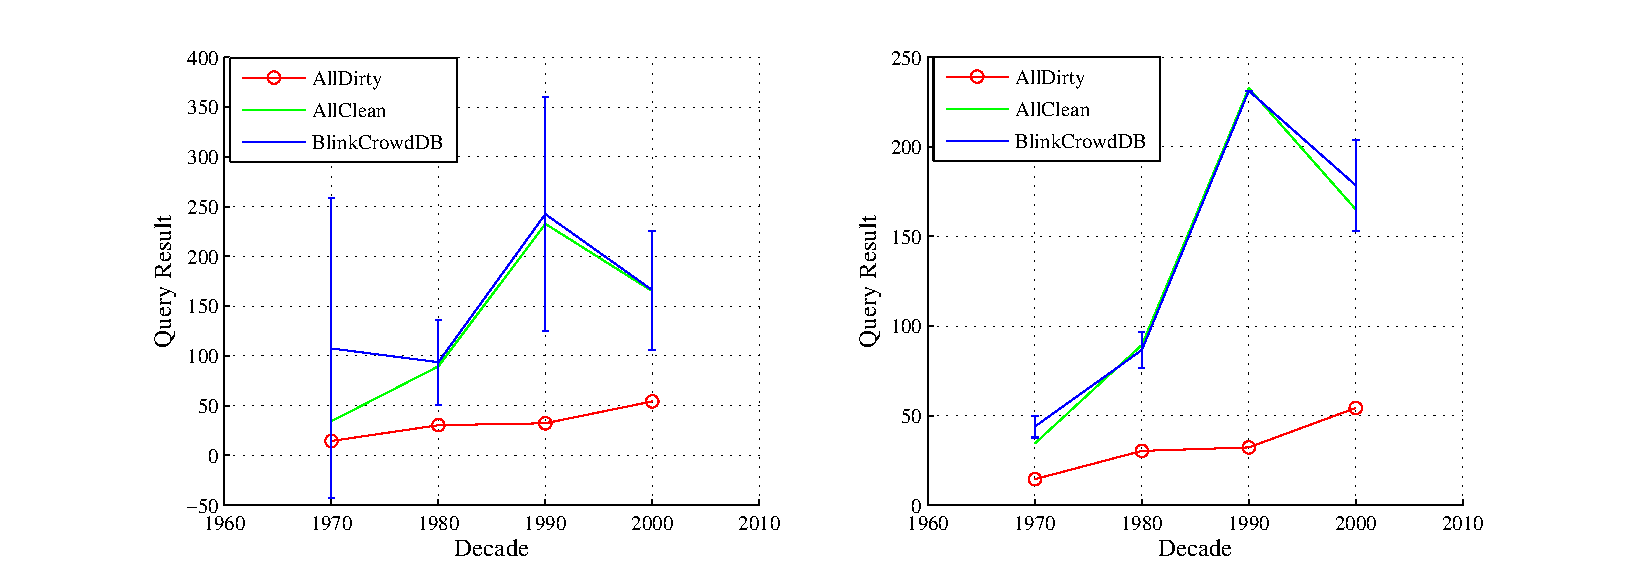
\includegraphics[scale=0.36]{exp/groupby-constraints.eps}\\
%\small {(a)500 tuples cleaned (b)1000 tuples cleaned}
%\caption{We calculated the mean citations for papers written in each decade, subject to cleaning constraints. Our estimates and confidence intervals are closer to the true value than an aggregation of the entire dirty data.}
%\label{exp:groupby-constraints}
%\vspace*{-10pt}
%\end{figure}
%We evaluated our query processing framework with \textbf{group by} queries with cost constraints on the MS Academic-Google Scholar Dataset.
%We ran the following two queries to calculate the mean number of citations per paper in each decade:
%\begin{alltt}
%SELECT \textsf{AVG}(CITATIONS) FROM Publication
%WHERE Conference = "\textsf{SIGMOD}"
%GROUP BY round(Year/10)
%WITHIN COST 500 TUPLES
%\end{alltt}

%\begin{alltt}
%SELECT \textsf{AVG}(CITATIONS) FROM Publication
%WHERE Conference = "\textsf{SIGMOD}"
%GROUP BY round(Year/10)
%WITHIN COST 1000 TUPLES
%\end{alltt}

%The results are shown in Figure \ref{exp:groupby-constraints}, and we can clearly see that the estimates and the confidence intervals outperform an aggregation of the entire dirty data.
%We can also see that increasing the budget reduces the maximum error by targeting the populations that have the biggest uncertainty.
%An important point is that the allocation algorithm is relatively sensitive to the initial estimates of variance.
%If we don't clean a sufficiently large constant sample of data to get an initial estimate of the error for each population, then the algorithm could give an allocation that is far from optimal.
